\documentclass[10pt,twocolumn]{article}
\topmargin=0.0in %length of margin at the top of the page (1 inch added by default)
\oddsidemargin=0.0in %length of margin on sides for odd pages
\evensidemargin=0in %length of margin on sides for even pages
\textwidth=6.5in %How wide you want your text to be
\marginparwidth=0.5in
\headheight=0pt %1in margins at top and bottom (1 inch is added to this value by default)
\headsep=0pt %Increase to increase white space in between headers and the top of the page
\textheight=9.1in %How tall the text body is allowed to be on each page

\usepackage{url}
\usepackage{graphicx}
\usepackage{authblk}
\usepackage{hyperref}
\usepackage{amsthm}
\usepackage{listings}
% "define" Scala
\lstdefinelanguage{scala}{morekeywords={class,object,trait,extends,with,new,if,while,for,def,val,var,this},
otherkeywords={->,=>},
sensitive=true,
morecomment=[l]{//},
morecomment=[s]{/*}{*/},
morestring=[b]"}
% Default settings for code listings
\lstset{frame=tb,language=scala,aboveskip=3mm,belowskip=3mm,showstringspaces=false,columns=flexible,basicstyle={\small\ttfamily}}

\theoremstyle{plain}

\widowpenalty=500
\clubpenalty=500
\setlength{\parskip}{3pt}

\date{}

\begin{document}

\title{ADAM: Genomics Formats and Processing Patterns for Cloud Scale Computing}
\author[1]{Matt~Massie}
\author[1]{Frank~Austin~Nothaft}
\author[1,2]{Chris~Hartl}
\author[1]{Christos~Kozanitis}
\author[3]{Andr\'{e}~Schumacher}
\author[1]{Anthony~D.~Joseph}
\author[1]{David~Patterson}
\affil[1]{Department of Electrical Engineering and Computer Science, University of California, Berkeley}
\affil[2]{The Broad Institute of MIT and Harvard}
\affil[3]{International Computer Science Institute, University of California, Berkeley}

\maketitle

\raggedbottom

\abstract

Current genomics applications are dominated by the movement of data to and from disk. This data movement pattern
is a significant bottleneck that prevents these applications from scaling well to distributed computing clusters. In this report,
we introduce a new set of data formats and programming patterns for genomics applications using in-memory MapReduce
frameworks. These formats and frameworks improve application performance, data storage efficiency, and programmer productivity.

\section{Introduction}
\label{sec:introduction}

Although the cost of data processing has not historically been an issue for genomic studies, the falling cost of genetic
sequencing will soon turn computational tasks into a dominant cost~\cite{nhgri}. The process of transforming reads
from alignment to variant-calling ready reads involves several processing stages including duplicate marking, base
score quality recalibration, and local realignment. Currently, these stages have involved reading a Sequence/Binary
Alignment Map~(SAM/BAM) file, performing transformations on the data, and writing this data back out to disk as a
new SAM/BAM file~\cite{li09}.

Because of the amount of time these transformations spend shuffling data to and from disk, these transformations have become
the bottleneck in modern variant calling pipelines. It currently takes three days to perform these transformations on a high
coverage BAM file\footnote{A 250GB BAM file at 30$\times$ coverage. See~\S\ref{sec:applications} for a longer discussion}. By
rewriting these applications to make use of modern in-memory MapReduce frameworks like Apache Spark~\cite{zaharia10}, these
transformations can now be completed in under two hours. Sorting and duplicate mapping alone can be accelerated to take
50 minutes on a commodity cluster. The format we present also provides many programming efficiencies, as it is easy to
change evidence access techniques, and is directly portable across many programming languages.

In this paper, we introduce ADAM, which is a programming framework and a set of data formats for cloud scale genomic
processing. These frameworks and formats scale efficiently to modern cloud computing performance, which allows us to
parallelize read translation steps that are required between alignment and variant calling. In this paper, we provide an
introduction to the data formats~(\S\ref{sec:current-genomics-storage-standards}) and pipelines used to process
genomes~(\S\ref{sec:genomic-processing-pipelines}), introduce the ADAM formats and data access
application programming interfaces~(APIs)~(\S\ref{sec:data-format-and-api}) and programing
model~(\S\ref{sec:in-memory-programming-model}). Finally, we review the performance and compression gains we
achieve~(\S\ref{sec:performance}), and outline future enhancements to ADAM that we are working on~(\S\ref{sec:future-work}).

\section{Current Genomics Storage Standards}
\label{sec:current-genomics-storage-standards}

The current de facto standard for the storage and processing of genomics data in read format is BAM. BAM is a binary file
format that implements the SAM standard for read storage~\cite{li09}. BAM files can be operated on in several languages,
using either the SAMtools~(\cite{li09}, C++), Picard~(\cite{picard}, Java), and Hadoop-BAM~(\cite{niemenmaa12}, Hadoop
MapReduce through Java) APIs. BAM provides more efficient access and compression than the SAM file format, as its binary
encoding reduces several fields into a single byte, and eliminates text processing on load. However, the file format has been
criticized as it is difficult to process --- the three main APIs that implement the format each note that they do not fully implement
the format due to its complexity. Additionally, the file format is difficult to use in multiprocessing environments due to its use
of a centralized header; the Hadoop-BAM implementation notes that it's scalability is limited to distributed processing
environments of less than 8 machines.

In response to the growing size of sequencing files\footnote{High coverage BAM files can be approximately 250 GB for a human genome.},
a variety of compression methods have come to light~\cite{kozanitis2011, fritz11, WanBioinformatics, Popitsch2012, Asnani2012, CoxBW, 
recoil, Jones2012, Janin2013}. SlimGene~\cite{kozanitis2011}, cSRA~\cite{SRA}, and CRAM~\cite{fritz11} use reference based compression
techniques to losslessly represent reads while they advocate in favor of lossy quality value representations. The former two use lower
quantization levels to represent quality values and CRAM uses user defined budgets to store only fractions of a quality string. 
In the same spirit, Illumina presented recently a systematic approach of quality score removal in~\cite{Janin2013} which safely ignores
quality scores from predictable nucleotides; these are bases that always appear after certain words. It is also worth mentioning that the
standard configurations of cSRA and CRAM discard the optional fields of the BAM format and also simplify the QNAME field. 

\section{Genomic Processing\\Pipelines}
\label{sec:genomic-processing-pipelines}

After sequencing and alignment, there are a few common steps in modern genomic processing pipelines for producing
variant call ready reads. These steps minimize the amount of erroneous data in the input read set by eliminating duplicate data,
verifying the alignment of short inserts/deletions~(indels), and calibrating the quality scores assigned to bases~(base quality score
recalibration, BQSR). The typical pipeline for variant calling is illustrated in figure~\ref{fig:pipeline}.

\begin{figure}[h]
\begin{center}
\includegraphics[width=0.9\linewidth]{pipeline.pdf}
\end{center}
\caption{Variant Calling Pipeline}
\label{fig:pipeline}
\end{figure}

Traditionally, bioinformaticians have focused on improving the accuracy of the algorithms used for alignment and variant
calling. There is obvious merit to this approach~---~these two steps are the dominant contributors to the accuracy of the variant
calling pipeline. However, the intermediate read processing stages are responsible for the majority of execution time. A
breakdown of stage execution time is shown in table~\ref{tab:stage-time} for the version 2.7 of the Genome Analysis
Toolkit~(GATK), a popular variant calling pipeline~\cite{mckenna10}. The numbers in the table are derived from running on
the NA12878 high-coverage human genome.

\begin{table}[h]
\caption{Processing Stage Times for GATK Pipeline}
\label{tab:stage-time}
\begin{center}
\begin{tabular}{| l | c | c |}
\hline
\bf Stage & \bf GATK 2.7/NA12878 \\
\hline
Mark Duplicates & 13 hr \\
BQSR & 9 hr \\
Realignment & 32 hr \\
Call Variants & 8 hr \\
\bf Total & \bf 64 hr \\
\hline
\end{tabular}
\end{center}
\end{table}

To provide the readers with a background about how the stages of this pipeline work, we will discuss the algorithms that
implement the intermediate read processing stages. For a detailed discussion of these algorithms, we refer readers to DePristo
et al~\cite{depristo11}.

\paragraph{Sorting:}
\label{sec:sorting}

This phase performs a pass over the reads and sorts them by the reference position at the start of their alignment.

\paragraph{Duplicate Removal:} 
\label{sec:duplicate-removal}

An insufficient number of sample molecules immediately prior to PCR can cause the generation of duplicate DNA sequencing reads.
Detection of duplicate reads requires matching all reads by their 5$'$ position and orientation after read alignment. Reads with
identical position and orientation are assumed to be duplicates. When a group of duplicate reads is found, each read is scored
and all, but the top-scoring read, are marked as duplicates. Approximately 66\% of duplicates marked in this way are true
duplicates caused by PCR-induced duplication while the remaining 33\% are caused by the random distribution of read ends\cite{20565776}.
There is currently no way to separate "true" duplicates from randomly occurring duplicates.

\paragraph{Base Quality Score Recalibration:} 
\label{sec:bqsr}

During the sequencing process, systemic errors occur that lead to the incorrect assignment of base quality scores. In this step, a
statistical model of the quality scores is built and is then used to revise the measured quality scores.

\paragraph{Local Realignment:} 
\label{sec:local-realignment}

For performance reasons, all modern aligners use algorithms that provide approximate alignments. This can cause reads with
evidence of indels to have slight misalignments with the reference. In this stage, we use fully accurate sequence alignment
methods~(Smith-Waterman algorithm~\cite{smith81}) to locally realign reads that contain evidence of short indels. This pipeline
step is omitted in some variant calling pipelines, if the variant calling algorithm that is implemented is not susceptible to these
local alignment errors.

For current implementations of these read processing steps, performance is limited by disk bandwidth. This is because the operations
read in a SAM/BAM file, perform a bit of processing, and write the data to disk as a new SAM/BAM file. We address this by performing
our processing iteratively in memory. The four read processing stages can then be chained together, eliminating three dumps to
disk and an additional three long reads from disk. The stages themselves cannot be performed in parallel, but the operations inside each
stage are data parallel. 

\section{Design Philosophy}
\label{sec:design-philosophy}

Modern bioinformatics pipelines have been designed without a model for how the system should grow or for how
components of the analytical system should connect. We seek to provide a more principled model for system composition.
Our system architecture was inspired heavily by the Open Systems Interconnection (OSI) model for networking
services~\cite{zimmermann80}. This conceptual model standardized the internal functionality of a networked
computer system, and its "narrow waisted" design was critical to the development of the services that would
become the modern internet. We present a similar decomposition of services for genomics data in
figure~\ref{fig:stack-model}.

\begin{figure}[h]
\begin{center}
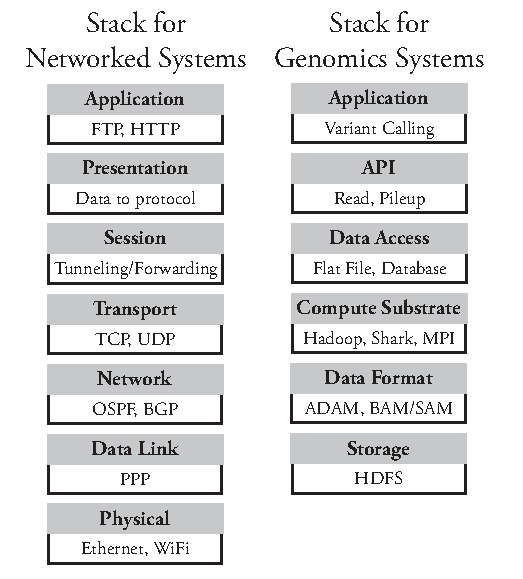
\includegraphics[width=0.6\linewidth]{stack-model.pdf}
\end{center}
\caption{Stack Models for Networking and Genomics}
\label{fig:stack-model}
\end{figure}

The seven levels of our stack model are decomposed as follows:

\begin{enumerate}
\item {\bf Physical Storage:} This layer coordinates data writes to physical media.
\item {\bf Storage:} This layer manages access, replication, and distribution of the genomics files that have been written to disk.
\item {\bf Materialized Data:} This layer encodes the patterns for how data is encoded and stored. This provides read/write efficiency
and compression.
\item {\bf Data Schema:} This level specifies the representation of data when it is accessed, and forms the narrow waist of the pipeline.
\item {\bf Evidence Access:} This layer implements efficient methods for performing common access patterns such as random database
queries, or sequentially reading records from a flat file.
\item {\bf Presentation:} The presentation layer sits on top of the data access layer and provides the application developer with efficient and
straightforward methods for querying the characteristics of individual portions of genetic data.
\item {\bf Application:} Applications like variant calling and alignment are implemented in this layer.
\end{enumerate}

A well defined software stack has several significant advantages. By limiting application interactions with layers lower than the API,
application developers are given a clear and consistent view of the data they are processing. By divorcing the API from the data
access layer, we unlock significant flexibility. With careful design in the data format and data access layers, we can seamlessly
support conventional flat file access patterns, while also allowing easy access to data with database
methods~(see~\S\ref{sec:database-integration}). By treating the compute substrate and storage as separate layers, we also
drastically increase the portability of the APIs that we implement. This approach is a significant improvement over current approaches
which intertwine all layers together --- if all layers are intertwined, new APIs must be developed to support new compute
substrates~\cite{niemenmaa12}, and new access patterns must be carefully retrofitted to the data format that is in use~\cite{kozanitis13}.

We can distill our philosophy into three observations that drive our design decisions:

\begin{enumerate}
\item {\bf Scalability is a primary concern for modern genomics systems:} Processing pipelines operate on data that can range in size from
tens of gigabytes to petabytes. We cannot remove processing stages, as this has an unacceptable impact on accuracy. To increase
pipeline latency and throughput, our systems must be able to parallelize efficiently to tens to hundreds of compute nodes.
\item {\bf Bioinformaticans should be concerned with data, not formats:} The SAM/BAM formats do not provide a schema for the data they
store. This limits visibility into the structure of data being processed. Additionally, it significantly increases implementation difficulty: by
making the format a primary concern, significant work has been required to introduce programming interfaces that allow these formats to
be read from different programming languages and environments~\cite{li09,picard,niemenmaa12}.
\item {\bf Openness and flexibility are critical to adoption:} As the cost of sequencing continues to drop~\cite{nhgri}, the processing of genomics
data will become more widespread. By maintaining an open source standard that can be flexibly modified, we allow all the members of the
community to contribute to improving our technologies. Developing a flexible stack is also important; genetic data will be processed in a host
of heterogenous computing environments, and with a variety of access patterns. By making our format easy to adopt to different techniques, we
maximize its use.
\end{enumerate}

In the next few sections, we discuss the implementation of ADAM, and how it was designed to satisfy these goals. We then
analyze the performance of our system and discuss the greater impact of our design philosophy. We believe that the greatest contribution of
our stack design is the explicit schema we have introduced. This alone drives the flexibility of the stack: on top of a single exposed schema, it
is trivial to change the evidence access layer to represent the relevant data in array, or tabular form. This is essential, as it makes it inexpensive
to support novel access patterns, which can enable new algorithms and applications.

\section{Data Format and API}
\label{sec:data-format-and-api}

ADAM contains formats for storing read and reference oriented sequence information, and variant/genotype data.
The read oriented sequence format is forwards and backwards compatible with BAM/SAM, and the variant/genotype
data is forwards and backwards compatible with VCF. In this section, we discuss the frameworks used to store this
data. We then introduce the representations, and discuss the content of each representation.

The data representation for the ADAM format is described using the open source Apache Avro data serialization
system~\cite{avro}. The Avro system also provides a human readable schema description language that can
auto-generate the schema implementation in several common languages including Scala, Java, C/C++/C\#,
Python, Ruby, and php. This provides a significant cross-compatibility advantage over the BAM/SAM format,
where the data format has only been implemented for C/C++ through Samtools and for Java through
Picard~\cite{li09,picard}. To complicate matters, there are well known incompatibilities between these different APIs,
as well as APIs for accessing variant data~(discussed in~\S\ref{sec:variant-and-genotype-storage}).

We layer this data format inside of the Parquet column store~\cite{parquet}. Parquet is an open source columnar storage
format that was designed by Cloudera and Twitter, which can be used as a single flat file, a distributed file, or as a database inside of Hive, Shark, or Impala. Columnar stores like Parquet provide several significant advantages when storing genomic data:

\begin{itemize}
\item Column stores enable predicate pushdown~\cite{lamb12}, which minimizes the amount of data read from disk. When
using predicate pushdown, we deserialize specific fields in a record from disk, and apply them to a predicate function. We
then only read the full record if it passes the predicate. This is useful when implementing filters that check read quality.
\item Column stores achieve extremely high compression~\cite{abadi06}. This reduces storage space on disk, and also improves
serialization performance inside of MapReduce frameworks. We are able to achieve a 0.75$\times$ lossless compression
ratio when compared to BAM, and have especially impressive results on quality scores. This is discussed in more
detail in~\S\ref{sec:compression}.
\item Varied data projections can be achieved with column stores. This means that we can choose to only read several
fields from a record. This improves performance for applications that do not read all the fields of a record. Additionally,
we do not pay for null fields in records that we store. This allows us to easily implement lossy compression on top of the
ADAM format, and also allows us to eliminate the FASTQ standard.
\end{itemize}

By supporting varied data projections with low cost for field nullification, we can implement lossy compression on top
of the ADAM format. We discuss this further in~\S\ref{sec:compression}.

A visualization of how ADAM in Parquet compares with BAM can be seen in figure~\ref{fig:file-format}. We remove the file header
and instead distribute these values across all of the records stored. This eliminates global information and makes the file much
simpler to distribute across machines. This is effectively free in a columnar store, as the store just notes that the information is
replicated across many reads. Additionally, Parquet writes data to disk in regularly sized row groups~(from~\cite{parquet}, see
Parquet format readme)~---~this allows parallelism across rows by enabling the columnar store to be split into independent
groups of reads.

\begin{figure}[h]
\begin{center}
\includegraphics[width=\linewidth]{file-format.pdf}
\end{center}
\caption{Comparative Visualization of BAM and ADAM File Formats}
\label{fig:file-format}
\end{figure}

As discussed in~\S\ref{sec:design-philosophy}, the internal data types presented in this section make up the narrow waist of our
proposed genomics stack. In~\S\ref{sec:database-integration} and~\S\ref{sec:columnar-vs-row-storage}, we review how this
abstraction allows us to support different data access frameworks and storage techniques to tailor the stack for the needs of
a specific application.

\subsection{Read Oriented Storage}
\label{sec:read-oriented-storage}

Our default read oriented data format is defined in table~\ref{tab:read-oriented-format}. This format provides all of the
fields supported by the SAM format. To make it easier to split the file between multiple machines for distributed processing,
we have eliminated the file header. Instead, the data encoded in the file header can be reproduced from every single
record. Because our columnar store supports dictionary encoding and these fields are replicated across all records,
replicating this data across all records has a negligible cost in terms of file size on disk.

\begin{table}[h]
\caption{Read Oriented Format}
\label{tab:read-oriented-format}
\begin{center}
\begin{tabular}{| c | l | c |}
\hline
\bf Group & \bf Field & \bf Type \\
\hline
General & Reference Name & String \\
 & Reference ID & Int \\
 & Start & Long \\
 & Mapping Quality & Int \\
 & Read Name & String \\
 & Sequence & String \\
 & Mate Reference & String \\
 & Mate Alignment Start & Long \\
 & Mate Reference ID & Int \\
 & Cigar & String \\
 & Base Quality & String \\
\hline
Flags & Read Paired & Boolean \\
 & Proper Pair & Boolean \\
 & Read Mapped & Boolean \\
 & Mate Mapped & Boolean \\
 & Read Negative Strand & Boolean \\
 & Mate Negative Strand & Boolean \\
 & First Of Pair & Boolean \\
 & Second Of Pair & Boolean \\
 & Primary Alignment & Boolean \\
 & Failed Vendor Checks & Boolean \\
 & Duplicate Read & Boolean \\
\hline
Attributes & Mismatching Positions & String \\
 & Other Attributes & String \\
\hline
Read Group & Sequencing Center & String \\
 & Description & String \\
 & Run Date & Long \\
 & Flow Order & String \\
 & Key Sequence & String \\
 & Library & String \\
 & Median Insert & Int \\
 & Platform & String \\
 & Platform Unit & String \\
 & Sample & String \\
\hline
\end{tabular}
\end{center}
\end{table}

This format is used to store all data on disk. In addition to this format, we provide an enhanced API for accessing read
data.

\subsection{Reference Oriented Storage}
\label{sec:reference-oriented-storage}

In addition to storing sequences as reads, we provide a storage format for reference oriented (pileup) data. This format
is documented in table~\ref{tab:reference-oriented-format}. This pileup format is also used to implement a data storage
format similar to the GATK's ReducedReads format~\cite{depristo11}.

\begin{table}[h]
\caption{Reference Oriented Format}
\label{tab:reference-oriented-format}
\begin{center}
\begin{tabular}{| c | l | c |}
\hline
\bf Group & \bf Field & \bf Type \\
\hline
General & Reference Name & String \\
 & Reference ID & Int \\
 & Position & Long \\
 & Range Offset & Int \\
 & Range Length & Int \\
 & Reference Base & Base \\
 & Read Base & Base \\
 & Base Quality & Int \\
 & Mapping Quality & Int \\
 & Number Soft Clipped & Int \\
 & Number Reverse Strand & Int \\
 & Count At Position & Int \\
\hline
Read Group & Sequencing Center & String \\
 & Description & String \\
 & Run Date & Long \\
 & Flow Order & String \\
 & Key Sequence & String \\
 & Library & String \\
 & Median Insert & Int \\
 & Platform & String \\
 & Platform Unit & String \\
 & Sample & String \\
\hline
\end{tabular}
\end{center}
\end{table}

We treat inserts as an inserted sequence range at the locus position. For bases that are an alignment match against the
reference\footnote{Following the conventions for CIGAR strings, an alignment match does not necessarily correspond to
a sequence match. An alignment match simply means that the base is not part of an indel. The base may not match the
reference base at the loci.}, we store the read base and set the range offset and length to 0. For deletions, we perform the
same operation for each reference position in the deletion, but set the read base to null. For inserts, we set the range length
to the length of the insert. We step through the insert from the start of the read to the end of the read, and increment the
range offset at each position.

As noted earlier, this datatype supports an operation similar to the GATK's ReducedRead datatype. We refer to these datatypes
as aggregated pileups. We perform aggregation by grouping together all bases that share a common reference position and
read base. Within an insert, we group further by the position in the insert. Once the bases have been grouped together, we average
the base and mapping quality scores. We also count the number of soft clipped bases that show up at this location, and the amount
of bases that are mapped to the reverse strand.

\subsection{Variant and Genotype Storage}
\label{sec:variant-and-genotype-storage}

The VCF specification more closely resembles an exchange format than a data format. In particular, the per-site and per-sample fields
(``\textsc{Info}'' and ``\textsc{Format}'') define arbitrary key-value pairs, for which parsing information is stored in the header of the file.
This enables side computation (such as classifying a particular SNP as likely or unlikely to damage the structure of a protein) to operate on a VCF
and store their results. A typical analysis pipeline may comprise of several steps which read in the VCF produced by the previous step, add
additional annotations to the \textsc{Info} and \textsc{Format} fields, and write a new VCF.

Maintaining full compatibility with VCF presents a structural challenge. Each (properly constructed) VCF file contains the data schema for
its \textsc{Info} and \textsc{Format} fields within the file header; and potentially every VCF file utilizes a different schema. Maintaining support
for these catch-all fields by incorporating the file schema within an ADAM-VCF Record violates the layer separation that is a part of the design
goals: the Evidence Access layer would take on the role of reading format information from a record, and using that to parse the contents of an
information blob. Furthermore, the format information is ``hidden'' from the Schema layer: the system cannot know what information the record
should contain until it looks at the format information for the record. This presents challenges to tools, which cannot check whether a field they
expect is part of the record schema (until runtime), to developers (who will have to write their own parsers for these unstructured blobs), and to
repository maintainers who need to adjudicate whose (complex) fields and parsers are widely-used enough to merit inclusion and official support.

\begin{table}[h]
\caption{Genotype Format}
\label{tab:genotype-format}
\begin{center}
\begin{tabular}{| l | c |}
\hline
\bf Field & \bf Type \\
\hline
Sample ID & String \\
Reference Allele & String \\
Site Alleles & String \\
Allele 1 & String \\
Allele 2 & String \\
Expected 1 Dosage & String \\
Expected 2 Dosage & String \\
Genotype Quality & Int \\
Likelihood (Phred) & String \\
Posterior Likelihoods & String \\
Ploidy State Likelihoods & String \\
Is Phased & Boolean \\
Phase Switch & Boolean \\
Phase Set ID & String \\
Phase Likelihood & Double \\
Haplotype 1 Quality & Int \\
Haplotype 2 Quality & Int \\
RMS Mapping Quality & Double \\
Depth & Int \\
Ethnicity & String \\
Cohort & String \\
\hline
\end{tabular}
\end{center}
\end{table}

\begin{table}[h]
\caption{Variant Format}
\label{tab:variant-format}
\begin{center}
\begin{tabular}{| l | c |}
\hline
\bf Field & \bf Type \\
\hline
Domain IDs & String \\
Reference ID & String \\
Reference Name & String \\
Start Position & Long \\
Site ID & String \\
Site Quality & Double \\
Site Filter & String \\
Ancestral Allele & String \\
Allele Count & String \\
Allele Frequency & String \\
Allele Number & Int \\
RMS Base Quality & Double \\
Allellic Alignments & String \\
In dbSNP? & Boolean \\
In HM2? & Boolean \\
In HM3? & Boolean \\
In 1000G? & Boolean \\
Site RMS MapQ & Double \\
MapQ=0 Count & Int \\
Samples With Data & Int \\
Strand Bias & Double \\
Is Somatic? & Boolean \\
Validated? & Boolean \\
Callset IDs & String \\
Callsets Present & Int \\
Callsets Filtered & Int \\
Gene IDs & String \\
Transcript IDs & String \\
\hline
\end{tabular}
\end{center}
\end{table}

The ``narrow waist'' of the ADAM Schema divides the world of parsing and file formats from the world of data presentation and processing.
To further abuse the allegory of the network stack: just as the transport layer need not worry about how to retrieve data from across a network
boundary, the access layer of the bioinformatic process should not need to worry about parsing or formatting raw data blobs. The VCF format
has resulted repeated violations of this principle. While the VCF format is supposed to render a schema for all key value pairs in its \textsc{Info}
and \textsc{Format} fields, a number of bioinformatics tools do not provide this parsing information, and so types must be inferred. In addition,
some tools (in particular annotation tools such as VariantEffectPredictor\cite{vep}) serialize rich data types (such as nested maps) into the
\textsc{Info} field, describing their format as simply ``String''. By adhering rigidly to specific schema, not only do we encourage separation of
concerns, we also limit extensibility abuse, and the practice of looking at online documentation to understand how to parse a field in a VCF.
The schema is the documentation, and the parsing is not the tool writer's concern!

These issues extend beyond tools that produce malformed VCFs or uninterpretable schema; the format is ill-supported by APIs that intend to
support them. For instance, PyVCF always splits on commas, even if the number of values is defined as 1. Thus it mis-parses VariantPredictorOutput
which is a single (though doubly-delimited by ``,'' and ``|'') field. Similarly to facilitate compression, per-sample fields (are not required to propagate all values. 

\section{In-Memory Programming\\Model}
\label{sec:in-memory-programming-model}

As discussed in~\S\ref{sec:genomic-processing-pipelines}, the main bottleneck in current genomics processing pipelines is
packaging data up on disk in a BAM file after each processing step. While this process is useful as it maintains data
lineage\footnote{Since we store the intermediate data from each processing step, we can later redo all pipeline processing
after a certain stage without needing to rerun the earlier stages. This comes at the obvious cost of space on disk. This tradeoff
makes sense if the cost of keeping data on disk and reloading it later is lower than the cost of recomputing the data. This
does not necessarily hold for modern MapReduce frameworks~\cite{zaharia12}.}, it significantly increases the latency of the
processing pipeline.

For the processing pipeline we have built on top of the ADAM format, we have minimized disk accesses~(read one file at the
start of the pipeline, and write one file after all transformations have been completed). Instead, we cache the reads that we are
transforming in memory, and chain multiple transformations together. Our pipeline is implemented on top of the Spark MapReduce
framework, where reads are stored as a map using the Resilient Distributed Dataset~(RDD) primitive.

\section{Performance}
\label{sec:performance}

This section reviews performance metrics pertinent to the ADAM file format, and applications written on top of ADAM. Our performance
analysis is partitioned into three sections:

\begin{itemize}
\item {\bf \ref{sec:microbenchmarks}. Microbenchmarks:} In this section, we review several testcases that have little computation, and
review ADAM against Hadoop-BAM. This section looks to evaluate the disk access performance of ADAM. In this section, we are most
interested in validating scalability and building intuition for the efficiencies provided by variable projection and predicate pushdown.
\item {\bf \ref{sec:applications}. Applications:} The main goal of ADAM is to accelerate the read processing pipelines that were introduced
in~\S\ref{sec:genomic-processing-pipelines}. In this section, we review the throughput of our processing pipeline.
\item {\bf \ref{sec:compression}. Compression:} Here, we review the reductions in disk space that we are able to achieve when compared
against BAM. We also review how we can achieve further compression through aggregating pileup data, and how to implement both
lossy and reference-based compression top of ADAM.
\end{itemize}

\subsection{Microbenchmarks}
\label{sec:microbenchmarks}

To validate the performance of ADAM, we created several microbenchmarks. These microbenchmarks are meant to demonstrate
the pure read/write throughput of ADAM, and to show how the system scales in a cluster. To validate these benchmarks, we implemented
the relevant tests in both ADAM and Hadoop-BAM~\cite{niemenmaa12}, running on Spark on an Amazon Elastic Compute 2 (EC2)
cluster. We used the $m2.4xlarge$ instance type for all of our tests. This instance type is an 8 core memory optimized machine
with 68.4 Gibibytes (GiB) of memory per machine. We ran these benchmarks against HG00096, a low-coverage human genome (15 GB
BAM) from the 1,000 Genomes Project. The file used for these experiments can be found on the 1000 Genomes ftp site, \texttt{ftp.1000genomes.ebi.ac.uk} in directory 
\begin{small}\texttt{/vol1/ftp/data/HG00096/alignment/}\end{small}.

\subsubsection{Read/Write Performance}
\label{sec:read-write-performance}

The decision to use a columnar store was based off of the observation that most genomics applications are read-heavy. In this section,
we aim to quantify the improvements in read performance that we achieve by using a column store, and how far these gains can be
maximized through the use of projections.

\paragraph{Read Length and Quality:}
\label{sec:read-length-and-quality}

This microbenchmark scans all the reads in the file, and collects statistics about the length of the read, and the mapping quality score.
The results of this benchmark can be found in Figure~\ref{fig:length-quality}. Ideal speedup curves are plotted along with the speedup measurements.

\begin{figure}[h]
\begin{center}
\includegraphics[width=\linewidth]{microbenchmarks/length_and_quality_low_coverage.pdf}
\end{center}
\caption{Read Length and Quality Speedup for HG00096}
\label{fig:length-quality}
\end{figure}

The speedups in this graph are plotted relative to the single machine Hadoop-BAM run.

This benchmark demonstrates several things:

\begin{itemize}
\item ADAM demonstrates superior scalability over Hadoop-BAM. This is likely because ADAM files can be more evenly distributed across machines.
Hadoop-BAM must guess the proper partitioning when splitting files~\cite{niemenmaa12}. The Parquet file format that ADAM is based on is partitioned
evenly when it is written\cite{parquet}. This is critical for small files such as the one used in this test~---~in a 16 machine cluster, there is only 1 GB of
data per node, so imbalances on the order of the Hadoop file split size (128 MB) can lead to 40\% differences in loading between nodes.
\item Projections can significantly accelerate computation, if the calculation does not need all the data. By projecting the minimum dataset necessary
to calculate the target of this benchmark, we can accelerate the benchmark by $8\times$. Even a more modest projection leads to a $2\times$
improvement in performance.
\end{itemize}

\subsubsection{Predicate Pushdown}
\label{sec:predicate-pushdown}

Predicate pushdown is one of the significant advantages afforded to us through the use of Parquet	~\cite{parquet}. In traditional
pipelines, the full record is deserialized from disk, and the filter is implemented as a Map/Reduce processing stage. Parquet provides
us with predicate pushdown: we deserialize only the columns needed to identify whether the record should be fully deserialized. We
then process those fields; if they pass the predicate, we then deserialize the full record.

We can prove that this process requires no additional reads. Intuitively this is true as the initial columns read would need to be read
if they were to be used in the filter later. However, this can be formalized.

\newtheorem{predicate-read-conserving}{Theorem}

\begin{predicate-read-conserving}
Predicate pushdown requires no additional disk accesses.
\end{predicate-read-conserving}

\begin{proof}

If $R$ is the set of records to read, $Proj$ is the projection we are using, and $size(i,j)$ returns the amount
of data recorded in column $j$ of record $i$, the total data read without predicate pushdown is:

\begin{equation}
\label{eqn:no-predicate}
\sum_{m}^{R}{\sum_{i}^{Proj}size(m,i)}
\end{equation}

By using predicate pushdown, we reduce this total to:

\begin{equation}
\label{eqn:predicate}
\sum_{m}^{R}{\sum_{i}^{Pred}size(m,i)} + \sum_{n}^{R_{p=True}}{\sum_{i}^{Proj \setminus Pred}size(n,i)}
\end{equation}

$Pred$ represents the set of columns used in the predicate. The set $R_{p=True}$ represents the subset of records in $R$ that pass
the predicate function. We can show that  if no records fail the predicate~(i.e.~$R~=~R_{p=True}$), then equations \ref{eqn:no-predicate}
and \ref{eqn:predicate} become equal. This is because by definition $Proj~=~(Pred~\cup~(Proj~\setminus~Pred))$.

\end{proof}

In this section, we seek to provide an intuition for how predicate pushdown can improve the performance of actual genomics workloads.
We apply predicate pushdown to implement read quality predication, mapping score predication, and predication by chromosome. 

\paragraph{Quality Flags Predicate:}
\label{sec:quality-flags-predicate}

This microbenchmark scans the reads in a file, and filters out reads that do not meet a specified quality threshold. We use the following
quality threshold:

\begin{itemize}
\item The read is mapped.
\item The read is at its primary alignment position.
\item The read did not fail vendor quality checks.
\item The read has not been marked as a duplicate.
\end{itemize}

This threshold is typically applied as one of the first operations in any read processing pipeline.

\paragraph{Gapped Predicate:}
\label{sec:gapped-predicate}

In many applications, the application seeks to look at a region of the genome~(e.g. a single chromosome or gene). We include this
predicate as a proxy: the gapped predicate looks for 1 out of every $n$ reads. This achieves performance analogous to filtering
on a single gene, but provides an upper bound as we pay a penalty due to our predicate hits being randomly distributed.

To validate the performance of predicate pushdown, we ran the predicates described above on the HG00096 genome on a
single AWS $m2.4xlarge$ instance. The goal of this was to determine the rough overhead of predicate projection.

For the gapped predicate, our performance with sweeping $n$ can be found in Figure~\ref{fig:gapped-filter}.

\begin{figure}[h]
\begin{center}
\includegraphics[width=\linewidth]{microbenchmarks/gapped_predicate_low_coverage.pdf}
\end{center}
\caption{Gapped Predicate on HG00096}
\label{fig:gapped-filter}
\end{figure}

There are several conclusions to be drawn from this experiment:

\begin{itemize}
\item As is demonstrated by equation~(\ref{eqn:predicate}), we see the largest speedup when our predicate read set is significantly
smaller than our projection read set. For smaller projections, we see a fairly substantial reduction in speedup.
\item As the number of records that passes the predicate drops, the number of reads done to evaluate the predicate begins to become
a dominant term. This has one important implication: for applications that plan to access a very small segment of the data, accessing the
data as a flat file with a predicate is likely not the most efficient access pattern. Rather, if the predicate is regular, it is likely better to access
the data through a indexed database.
\end{itemize}

We additionally calculated the performance improvement that was achieved by using predicate pushdown instead of a Spark filter.
These results can be found in Table~\ref{tab:filter-vs-predicate}.

\begin{table}[h]
\caption{Predicate Pushdown Speedup vs. Filtering}
\label{tab:filter-vs-predicate}
\begin{center}
\begin{tabular}{| l | c  c c | c |}
\hline
\bf Predicate & \bf Min & \bf Avg & \bf Max & \bf Filtered \\
\hline
Locus & 1.19 & 1.17 & 0.94 & 3\% \\
Gapped, $n = 1$ & 1.0 & 1.0 & 1.01 & 0\% \\
Gapped, $n = 2$ & 1.22 & 1.27 & 1.29 & 50\% \\
Gapped, $n = 4$ & 1.31 & 1.42 & 1.49 & 75\% \\
Gapped, $n = 8$ & 1.37 & 1.58 & 1.67 & 87.5\% \\
\hline
\end{tabular}
\end{center}
\end{table}

These results are promising, as they indicate that predicate pushdown is faster than a Spark filter in most cases. We believe that the
only case that showed a slowdown (max projection on Locus predicate) is due to an issue in our test setup. We therefore can conclude
that filtering operations that can be performed statically at file load-in should be performed using predicate pushdown.

\subsection{Applications}
\label{sec:applications}

ADAM relies on Apache Spark for in-memory, map-reduce processing. At the heart of Spark is a programming construct,
called a Resilient Distributed Dataset (RDD), which represents a fault-tolerant collection of elements that are
operated on in parallel. Programming with an RDD is very similar to programming with any standard Scala collection
like \texttt{Seq} or \texttt{List}. This polymorphism allows developers to focus on the algorithm they're developing 
without concerning themselves with the details of distributed computation. The example code presented in this section
highlight the succinctness and expressiveness of Spark Scala code. While ADAM is currently written exclusively in 
Scala, Apache Spark also has Java and Python support.

For these applications to be run in a distributed fashion, the data needs to be loaded onto the Hadoop
Distribute File System (HDFS). HDFS breaks the file into blocks, distributes them across the cluster and maintains
information about block (and replica) locations. Breaking large files, like BAM files, into blocks allows systems,
like Spark, to create tasks which run across the entire cluster processing the records inside of each block. 
The wall clock times presented in the applications below do not consider the time it takes to load data to HDFS.

The NA12878 high-coverage BAM file used for these experiments can be found on the 1000 Genomes ftp site, \texttt{ftp.1000genomes.ebi.ac.uk} in directory 
\begin{small}\texttt{/vol1/ftp/data/NA12878/high\_coverage\_alignment/}\end{small}.

\subsubsection{Flagstat}
\label{sec:flagstat}

Even the simplest application can benefit from the ADAM format and execution
environment. For example, the samtools \texttt{flagstat} command prints
read statistics on a BAM file, e.g.

\begin{scriptsize}
\begin{verbatim}
$ samtools flagstat NA12878.bam
1685229894 + 0 in total (QC-passed reads + QC-failed reads)
0 + 0 duplicates
1622164506 + 0 mapped (96.26\%:-nan\%)
1685229894 + 0 paired in sequencing
842614875 + 0 read1
842615019 + 0 read2
1602206371 + 0 properly paired (95.07\%:-nan\%)
1611286771 + 0 with itself and mate mapped
10877735 + 0 singletons (0.65\%:-nan\%)
3847907 + 0 with mate mapped to a different chr
2174068 + 0 with mate mapped to a different chr (mapQ>=5)
\end{verbatim}
\end{scriptsize}

ADAM has a \texttt{flagstat} command which provides 
identical information in the same text format.

\begin{table}[h]
\caption{Time to Run Flagstat on High-Coverage NA12878}
\label{tab:time-flagstat}
\begin{center}
\begin{tabular}{| l | c | c |}
\hline
\bf Software  & \bf Wall clock time \\
\hline
Samtools 0.1.19 & 25m24s \\ 
ADAM 0.5.0 & 0m46s \\
\hline
\end{tabular}
\end{center}
\end{table}

The ADAM \texttt{flagstat} command was run on EC2 with 32 \texttt{cr1.8xlarge} machines
which is, not suprisingly, why ADAM ran 34 times faster. While the samtools \texttt{flagstat}
command is multi-threaded, it can only be run on a single machine.

\subsubsection{Sort}
\label{sec:sort}

When coordinate sorting a BAM file, reads are reordered by reference id and alignment start position.
This sorting makes it easier for downstream tools to find reads for a specific area of the reference
and makes finding mates in paired-ends reads more efficient. Many utilities will only except 
BAM files that have been sorted, e.g. Picard MarkDuplicates.

Each read is mapped to a tuple with the two values: position and read.
Unmapped reads that a value of \texttt{None} for \texttt{ReferencePosition}
are sent to the end of the file.

\begin{table}[h]
\caption{Sort NA12878}
\label{tab:time-flagstat}
\begin{scriptsize}
\begin{center}
\begin{tabular}{| l | c | c |}
\hline
\bf Software & \bf EC2 profile & \bf Wall clock time \\
\hline
Picard Tools 1.102 & --- & 13h \\
ADAM 0.5.0 & 32 \texttt{cr1.8xlarge} & 32m38s \\
ADAM 0.5.0 & 100 \texttt{m2.4xlarge} & 20m57s \\ 
\hline
\end{tabular}
\end{center}
\end{scriptsize}
\end{table}

ADAM was run on an EC2 cluster with 32 \texttt{cr1.8xlarge} machines and
a cluster with 100 \texttt{m2.4xlarge} instances.

Monitoring the Spark console during sorting revealed that the \texttt{sortByKey}
operation (on line 10 above) took a total of 1 min 37 secs. The \texttt{map} operation
(at line 2 above) took 1 min 48 secs, and the remainder of the time, 29 min 25 secs, was 
spent writing the results to HDFS. There were a total of 1586 tasks with a majority
finishing in under 10 minutes. A sole traggling task took 29 min 25 secs to write
all unmapped reads. This indicates that using a custom partitioner could dramatically
improve performance.

\subsubsection{Mark Duplicates}
\label{sec:mark-duplicates}

The ADAM algorithm for marking duplicate is nearly identical to Picard's MarkDuplicates
command. 

\begin{table}[h]
\caption{Mark Duplicates for NA12878}
\label{tab:time-mark-duplicates}
\begin{scriptsize}
\begin{center}
\begin{tabular}{| l | c | c |}
\hline
\bf Software & \bf EC2 profile & \bf Wall clock time \\
\hline
Picard 1.102 & --- & 13h \\
ADAM 0.5.0 & 100 \texttt{m2.4xlarge} & 28m17 \\
\hline
\end{tabular}
\end{center}
\end{scriptsize}
\end{table}

Due to caching effects, we see a 20\% improvement in performance when we cascade Sort and Mark Duplicates together.

\begin{table}[h]
\caption{Sort and Mark Duplicates for NA12878}
\label{tab:time-mark-duplicates-sort}
\begin{scriptsize}
\begin{center}
\begin{tabular}{| l | c | c |}
\hline
\bf Software & \bf EC2 profile & \bf Wall clock time \\
\hline
Picard Tools 1.102 & --- & 26h \\
ADAM 0.5.0 & 100 \texttt{m2.4xlarge} & 50m45s \\
\hline
\end{tabular}
\end{center}
\end{scriptsize}
\end{table}

\subsection{Tuning Spark on EC2}

All applications were run on Amazon EC2 with minimal tuning. The performance numbers in this report
should not be considered best case performance numbers.

An important Apache Spark property is \texttt{spark.default.parallelism} which controls the number
of tasks to use for distributed shuffle operations. This value needs to be tuned to match the
underlying cluster that Spark is running on.

\begin{table}[h]
\caption{Time to Sort NA12878}
\label{tab:time-sort-parallelism}
\begin{center}
\begin{tabular}{| l | c | c |}
\hline
\bf \small{spark.default.parallelism} & \bf Wall clock time \\
\hline
500 & 47 min 10 secs \\
48 & 32 min 38 secs \\ 
\hline
\end{tabular}
\end{center}
\end{table}

The following graph shows CPU time series for two sort operations on a 32-node \texttt{cr1.8xlarge}
EC2 cluster running back to back with different values for \texttt{spark.default.parallelism}.
The early CPU profile is when \texttt{spark.default.parallelism} is set to 500 and the latter profile
is when it's set to 48. You can see from the graph that with the higher level of parallelism
there is a significantly higher amount of system CPU (in red) as 32 CPUs contend for access to 
the two disks in each \texttt{cr1.8xlarge} instance. While \texttt{cr1.8xlarge} instances provide
plenty of memory, they do not have enough disks to help spread the I/O load around.

\begin{figure}[h]
\begin{center}
\includegraphics[width=0.9\linewidth]{images/Ganglia CPU Graph.png}
\end{center}
\caption{Comparison of 500 to 48 parallelism}
\label{fig:parallelism}
\end{figure}

\subsection{Compression}
\label{sec:compression}

By using dictionary coding, run length encoding with bit-packing, and GZIP compression, ADAM files can be stored using less
disk space than an equivalent BAM file. Typically, ADAM is approximately 75\% of the size of the compressed BAM for the
same data. If one is performing pileup aggregation, compression can improve to over 50\%.

\section{Future Work}
\label{sec:future-work}

Beyond the initial release of the ADAM data formats, API, and read transformations, we are working on several other
extensions to ADAM. These extensions strive to make ADAM accessible to more users and to more programming patterns.

\subsection{Database Integration}
\label{sec:database-integration}

ADAM format plays a central role in a library that we develop which will allow sequencing data to be queried from 
the popular SQL based warehouse software such as Shark~\cite{shark}, Hive~\cite{hive} and Impala~\cite{impala}. In fact,
the Avro/Parquet storage backend enables the direct usage of ADAM files as SQL tables; this integration is facilitated through libraries 
that integrate Parquet with the aforementioned software~\cite{parquet}.

Of course there is a lot of work remaining before SHARK provides biologically relevant functionality,
such as the one that is outlined in Bafna et al~\cite{bafna2013}; Shark needs to be enhanced with libraries that provide
efficient indexing, storage management and interval query handling. The indexing scheme that we develop enables
range based read retrieval, such as the indexing mechanism of samtools, quick access to mate pair reads such as the
indexing mechanism of GQL~\cite{kozanitis13} and also text based search features on fields such as the read sequence
and the CIGAR string. To keep storage under control we implement a set of heuristics that prevent the materialization of
queries with reproducible output. Finally, given that most biological data is modelled after intervals on the human genome,
our library includes user defined functions that implement interval operators such as the IntervalJoin operator of GQL.

\subsection{API Support Across Languages}
\label{sec:api-support-across-languages}

Currently, the ADAM API and example read processing pipeline are implemented in the Scala language. However, long
term we plan to make the API accessible to users of other languages. ADAM is built on top of Avro, Parquet, and Spark.
Spark has bindings for Scala, Java, and Python, and Parquet implementations exist for Java and C++. As the data model
is implemented on top of Avro, the data model can also be auto\-generated for C/C++/C\#, Python, Ruby, and php. We hope
to make API implementations available for some of these languages at a later date.

\section{Discussion}
\label{sec:discussion}

As discussed in this paper, ADAM presents a significant jump for genomics data processing. To summarize, the benefits are as
follows:

\begin{itemize}
\item ADAM achieves approximately a $30\times$ speedup when compared to other modern processing pipelines.
\item ADAM can successfully scale to clusters larger than 100 nodes.
\item ADAM presents an explicit data schema which makes it straightforward for the data access layer to be changed
to support new access patterns.
\end{itemize}

In this section, we discuss a few tradeoffs inherent to ADAM, as well as new applications enabled by ADAM.

\subsection{Columnar vs. Row Storage}
\label{sec:columnar-vs-row-storage}

In our current implementation, we use the Parquet columnar store to implement the data access layer. We chose to use
columnar storage as we believe that columnar storage is a better fit for bioinformatics workloads than flat row storage;
this discussion is introduced in~\S\ref{sec:data-format-and-api}. Typically, column based storage is preferable unless
our workload is write heavy; write heavy workloads perform better with row based storage formats~\cite{stonebraker05}.
Genomics pipelines tend to skew in favor of reading data~---~pipelines tend to read a large dataset, prune/reduce data,
perform an analysis, and then write out a significantly smaller file that contains the results of the analysis.

However, it is conceivable that emerging workloads could change to be write heavy. We note that although our current
implementation would not be optimized for these workloads, the layered model proposed in~\S\ref{sec:design-philosophy}
allows us to easily change our implementation. Specifically, we can swap out columnar storage in the data access layer with
row oriented storage~\footnote{It is worth noting that the Avro serialization system that we use to define ADAM is a performant
row oriented system.}. The rest of the implementation in the system would be isolated from this change: algorithms in the
pipeline would be implemented on top of the higher level API, and the compute substrate would interact with the data access
layer to implement the process of reading and writing data.

\subsection{New Applications Enabled\\By ADAM}
\label{sec:new-applications}

The ADAM format and environment provides a significant performance improvement over current BAM based solutions. By reducing
processing latency, ADAM will make genomic data available for use in latency-critical applications, such as genomic driven treatment
of acute diseases. Additionally, the genomics stack design we proposed in~\S\ref{sec:design-philosophy} unlocks new computational
patterns that can be applied to genomic data. In this section, we introduce a few of these novel applications, discuss why they are important,
and explain how these applications are enabled by ADAM.

\subsubsection{Personalized Treatment of\\Acute Diseases}
\label{sec:personalized-acute-diseases}

There is significant interest in using genomic data as another layer of evidence for the treatment of diseases that have genetic
causes~\cite{ghosh09, van13}. While chronic hereditary diseases like Huntington's Disease may not be sensitive to the latency of genomic
processing pipelines, reduced latency is critical for neonatal diagnosis and for the treatment of some cancers. In acute myeloid
leukemia~(AML), there exists a well defined set of mutations that can be used for guiding patient treatment~\cite{smith12}. However,
due to the rapid progression of AML, treatment decisions must be made in under one week. As illustrated
in~\S\ref{sec:genomic-processing-pipelines}, this target is not within the reach of current processing pipelines.

It is worth noting that the numbers presented in~\S\ref{sec:genomic-processing-pipelines} would be optimistic in reality. To improve
accuracy, the current state of the art in mutation calling uses very high coverage sequencing data~($\sim100-150\times$) for the
tumor cell line, along with high coverage sequencing data~($\sim30\times$) for the normal cell line~\cite{cibulskis13}. We are
developing a variant and mutation calling pipeline that uses the ADAM processing pipeline and the high-performance SNAP
aligner~\cite{zaharia11} to achieve performance that will satisfy the latency requirements for use in acute disease diagnosis.

\subsubsection{Viral Outbreak Monitoring}
\label{sec:viral-outbreak-monitoring}

There is significant interest in tools for the analysis of viral outbreaks in both the medical and defense epidemiology
communities~\cite{snitkin12,beard08}. Genomic techniques can be used for identifying infection vectors in epidemics that
feature rapidly mutating diseases, as well as for the rapid identification of unknown infectious agents in an attack using
biological weapons. Similar to the acute genetic driven diseases discussed in \S\ref{sec:personalized-acute-diseases}, both
of these applications are latency sensitive; the United States Department of Defense (DoD) has set a goal of developing a
system which can identify an unknown infectious agent within one hour with the use of genomic data.

In addition to providing significantly lower latency than current pipelines, there are other advantages to ADAM. Current
approaches to tracking viral outbreaks perform a graph based analysis that uses variant data and temporal data to identify
possible modes of disease transmission~\cite{snitkin12}. As ADAM is implemented on top of Spark, data in ADAM format
can be processed as a graph by using the GraphX distributed graph analysis framework~\cite{xin13}.

\subsubsection{Ad Hoc Genomic Analysis}
\label{sec:ad-hoc-genomic-analysis}

ADAM is implemented on top of the Spark MapReduce framework. A major contribution of the Spark framework was the introduction
of a command line interface that allows for the real-time ad hoc analysis of data kept in memory~\cite{zaharia12}. This interactive
framework can be coupled with the ability to perform interactive queries in Shark to allow for rapid data aggregation and analysis.
Several applications for this approach are presented by Kozanitis et al.~\cite{kozanitis13} such as allowing direct evidence access
to physicians who are working in a clinical setting with patients with hereditary diseases. However, GQL performance limited the
performance of these queries to $\sim45$ minutes. We are still working on the implementation of our database
interface~(see~\S\ref{sec:database-integration}), but expect to achieve improved performance.

In addition to clinical applications, interactive data access could be applied to pathway analysis. Specifically, if a biologist has
genetic data for organisms who demonstrate a specific phenotype, interactive data processing could be used for correlating
lab observations with genotypes. Instead of genotyping the full genome/exome of all reference organisms, the raw reads for
all organisms could be aligned in stored in a database. Once lab measurements and cytological observations have allowed
the biologist to hypothesize that a specific pathway had failed, the database of raw reads could be queried for all genes of
interest~(genes that influence the pathway under study). This would lead to a significant reduction in the amount of genomic
data that needed to be processed, which would allow for interactive read processing and variant calling.

\subsection{Programming Model\\Improvements}
\label{sec:programming-model-improvements}

Beyond improving performance by processing data in memory, our programming model improves programmer efficiency.
We build our operations as a set of transforms that extend the RDD processing available in Spark. These transformations
allow a very straightforward programming model that has been demonstrated to significantly reduce code size~\cite{zaharia12}.
Additionally, the use of Scala, which is an object functional statically typed language that supports type inference couples
provides further gains.

Additional gains come from our data model. We expose a clear schema, and build an API that expands upon this schema
to implement commonly needed functions. This API represents level 6 in the stack we proposed in
section~\S\ref{sec:design-philosophy}. To reduce the cost of this API, we make any additional transformations from our
internal schema to the data types presented in our API lazy. This eliminates the cost of providing these functions if they are
not used. Additionally, if an additional transformation is required, we only pay the cost the first time the transformation is performed.

In total, these improvements can provide a $2\times$ improvement in programmer productivity. This is demonstrated through
GAParquet, which demonstrates some of the functionality in the GATK on top of the ADAM stack~\cite{gaparquet}. In the
DiagnoseTargets stage of GATK, the number of lines of code~(LOC) needed to implement the stage dropped from 400 to
200. We also see a reduction in lines of code needed to implement the read transformation pipeline described
in~\S\ref{sec:genomic-processing-pipelines}. A LOC comparison of GATK/GAParquet and the read transformation pipeline
is found in table~\ref{tab:lines-of-code}.

\begin{table}[h]
\caption{Lines of Code for ADAM and Original Implementation}
\label{tab:lines-of-code}
\begin{center}
\begin{tabular}{| l | c | c |}
\hline
\bf Application & \bf Original & \bf ADAM \\
\hline
\hline
\multicolumn{3}{| l |}{\bf GATK Diagnose Targets} \\
\hline
Walker & 326 & 134 \\
Subclass & 93 & 66 \\
\bf Total & \bf 419 & \bf 200 \\
\hline
%\hline
%\multicolumn{3}{| l |}{\bf Translation Pipeline} \\
%\hline
%BQSR & & \\
%Mark Duplicates & & \\
%Realign Indels & & \\
%Sort & & \\
%\bf Total & & \\
%\hline
\end{tabular}
\end{center}
\end{table}

\section{Summary}
\label{sec:summary}

In this technical report, we have presented ADAM which is a new data storage format and processing pipeline for
genomics data. ADAM makes use of efficient columnar storage systems to improve the lossless compression available
for storing read data, and uses in-memory processing techniques to eliminate the read processing bottleneck faced
by modern variant calling pipelines. On top of the file formats that we have implemented, we also present APIs that enhance
developer access to read, pileup, genotype, and variant data. We are currently in the process of extending ADAM to
support SQL querying of genomic data, and extending our API to more programming languages. ADAM promises
to improve the development of applications that process genomic data, by removing current difficulties with the extraction
and loading of data and by providing simple and performant programming abstractions for processing this data.

\appendix

\section{Availability}
\label{sec:availability}

The ADAM source code is available at Github at \url{http://www.github.com/bigdatagenomics/adam}, and the ADAM project website
is at \url{http://adam.cs.berkeley.edu}. Additionally, ADAM is deployed through Maven with the following dependency:

\begin{verbatim}
TBD
\end{verbatim}

At publication time, the current version of ADAM is 0.5.0. ADAM is open source and is released under the Apache 2
license.

\section{Algorithm Implementations}
\label{sec:algorithm-implentations}

As ADAM is open source, the source code for the system is freely available. However, the implementations of the algorithms
are not always trivial. In this section, we highlight the algorithms that underly our read processing pipeline.

\subsection{Sort Implementation}
\label{sec:sort-implementation}

The ADAM Scala code for sorting a BAM file is succinct and relatively 
easy to follow. It is provided below for reference.

\begin{lstlisting}
def adamSortReadsByReferencePosition():
    RDD[ADAMRecord] = {
  rdd.map(p => {
    val referencePos = ReferencePosition(p) match {
      case None =>
        // Move unmapped reads to the end
        ReferencePosition(Int.MaxValue,
          Long.MaxValue)
      case Some(pos) => pos
    }
    (referencePos, p)
  }).sortByKey().map(p => p._2)
}
\end{lstlisting}

\subsection{BQSR Implementation}
\label{sec:bqsr-implementation}

Base Quality Score Recalibration is an important early data-normalization step in the bioinformatics pipeline, and after alignment
it is the next most costliest step. Since quality score recalibration can vastly improve the accuracy of variant calls~---~particularly for
pileup-based callers like the UnifiedGenotyper or Samtools mpileup. Because of this, it is likely to remain a part of bioinformatics pipelines.

BQSR is also an interesting algorithm in that it doesn't neatly fit into the framework of map reduce (the design philosophy of the GATK).
Instead it is an embarrassingly parallelizable aggregate. The ADAM implementation is:

\begin{lstlisting}
def computeTable(rdd: Records, dbsnp: Mask) :
  RecalTable = {
  
  rdd.aggregate(new RecalTable)(
    (table, read) => { table + read },
    (table, table) => { table ++ table })
}
\end{lstlisting}

The ADAM implementation of BQSR utilizes the MD field to identify bases in the read that mismatch the reference. This enables
base quality score recalibration to be entirely reference-free, avoiding the need to have a central Fasta store for the human
reference. However, dbSNP is still needed to mask out positions that are polymorphic (otherwise errors due to real variation will
severely bias the error rate estimates).

\subsection{Indel Realignment\\Implementation}
\label{sec:indel-realignment-implementation}

Indel realignment is implemented as a two step process. In the first step, we identify regions that have evidence of an insertion or
deletion. After these regions are identified, we generate candidate haplotypes, and realign reads to minimize the overall quantity
of mismatches in the region. The quality of mismatches near an indel serves as a good proxy for the local quality of an alignment.
This is due to the nature of indel alignment errors: when an indel is misaligned, this causes a temporary shift in the read sequence
against the reference sequence. This shift manifests as a run of several bases with mismatches due to their incorrect alignment.

\subsubsection{Realignment Target Identification}
\label{sec:realignment-target-identification}

Realignment target identification is done by converting our reads into reference oriented ``rods''\footnote{Also known as pileups: a
group of bases that are all aligned to a specific locus on the reference.}. At each locus where there is evidence of an insertion or a
deletion, we create a \emph{target} marker. We also create a target if there is evidence of a mismatch. These targets contain the indel
range or mismatch positions on the reference, and the range on the reference covered by reads that overlap these sites.

After an initial set of targets are placed, we merge targets together. This is necessary, as during the read realignment process, all
reads can only be realigned once. This necessitates that all reads are members of either one or zero realignment targets. Practically,
this means that over the set of all realignment targets, no two targets overlap.

The core of our target identification algorithm can be found below.

\begin{lstlisting}
def findTargets (reads: RDD[ADAMRecord]):
    TreeSet[IndelRealignmentTarget] = {

  // convert reads to rods
  val processor = new Read2PileupProcessor
  val rods: RDD[Seq[ADAMPileup]] = reads.flatMap(
      processor.readToPileups(_))
    .groupBy(_.getPosition).map(_._2)

  // map and merge targets
  val targetSet = rods.map(
      IndelRealignmentTarget(_))
    .filter(!_.isEmpty)
    .keyBy(_.getReadRange.start)
    .sortByKey()
    .map(new TreeSet()(TargetOrdering) + _._2)
    .fold(new TreeSet()(TargetOrdering))(
      joinTargets)

  targetSet
}
\end{lstlisting}

To generate the initial unmerged set of targets, we rely on the ADAM toolkit's pileup generation utilities~(see~\-S\ref{sec:reference-oriented-storage}).
We generate realignment targets for all pileups, even if they do not have indel or mismatch evidence. We eliminate pileups that do not contain indels
or mismatches with a filtering stage that eliminates empty targets. To merge overlapping targets, we map all of the targets into a sorted set. This set
is implemented using Red-Black trees. This allows for efficient merges, which are implemented with the tail-call recursive \emph{joinTargets} function:

\begin{lstlisting}
@tailrec def joinTargets (                                                                                                                                                               
  first: TreeSet[IndelRealignmentTarget],                                                                                                                                                                
  second: TreeSet[IndelRealignmentTarget]):
    TreeSet[IndelRealignmentTarget] = {

  if (!TargetOrdering.overlap(first.last,
      second.head)) {
    first.union(second)
  } else {
    joinTargets (first - first.last +
      first.last.merge(second.head),
      second - second.head)
  }
}
\end{lstlisting}

As we are performing a fold on an RDD which is sorted by the starting position of the target on the reference sequence, we know a priori that the elements
in the ``first'' set will always be ordered earlier relative to the elements in the ``second'' set. However, there can still be overlap between the two sets, as this
ordering does not account for the end positions of the targets. If there is overlap between the last target in the ``first'' set and the first target in the ``second''
set, we merge these two elements, and try to merge the two sets again.

\subsubsection{Candidate Generation\\and Realignment}
\label{sec:candidate-generation-realignment}

Candidate generation is a several step process:

\begin{enumerate}
\item Realignment targets must ``collect'' the reads that they contain.
\item For each realignment group, we must generate a new set of candidate haplotype alignments.
\item Then, these candidate alignments must be tested and compared to the current reference haplotype.
\item If a candidate haplotype is sufficiently better than the reference, reads are realigned.
\end{enumerate}

The mapping of reads to realignment targets is done through a tail recursive function that performs a binary search across the sorted set of indel alignment targets:

\begin{lstlisting}
@tailrec def mapToTarget (read: ADAMRecord,                                                                                                                                                        
  targets: TreeSet[IndelRealignmentTarget]):
    IndelRealignmentTarget = {

  if (targets.size == 1) {
    if (TargetOrdering.equals (targets.head, read)) {
      targets.head
    } else {
      IndelRealignmentTarget.emptyTarget
    }
  } else {
    val (head, tail) = targets.splitAt(
      targets.size / 2)
    val reducedSet = if (TargetOrdering.lt(
        tail.head, read)) {
      head
    } else {
      tail
    }
    mapToTarget (read, reducedSet)
  }
}
\end{lstlisting}

This function is applied as a groupBy against all reads. This means that the function is mapped to the RDD that contains all reads. A new RDD is generated where all
reads that returned the same indel realignment target are grouped together into a list.

Once all reads are grouped, we identify new candidate alignments. However, before we do this, we left align all indels. For many reads that show evidence of a single
indel, this can eliminate mismatches that occur after the indel. This involves shifting the indel location to the ``left''\footnote{To a lower position against the reference
sequence.} by the length of the indel. After this, if the read still shows mismatches, we generate a new consensus alignment. This is done with the
\emph{generateAlternateConsensus} function, which distills the indel evidence out from the read.

\begin{lstlisting}
def generateAlternateConsensus (sequence: String,
  start: Long, cigar: Cigar): Option[Consensus] = {
  var readPos = 0
  var referencePos = start

  if (cigar.getCigarElements.filter(elem =>
        elem.getOperator == CigarOperator.I ||
        elem.getOperator == CigarOperator.D
      ).length == 1) {
    cigar.getCigarElements.foreach(cigarElement =>
      { cigarElement.getOperator match {
        case CigarOperator.I => return Some(
          new Consensus(sequence.substring(readPos,
            readPos + cigarElement.getLength),
            referencePos to referencePos))
        case CigarOperator.D => return Some(
          new Consensus("",
          referencePos until (referencePos +
            cigarElement.getLength)))
        case _ => {
          if (cigarElement.getOperator
                .consumesReadBases &&
              cigarElement.getOperator
                .consumesReferenceBases
              ) {
            readPos += cigarElement.getLength
            referencePos += cigarElement.getLength
          } else {
            return None
          }
        }
      }
    })
    None
  } else {
    None
  }
}
\end{lstlisting}

From these consensuses, we generate new haplotypes by inserting the indel consensus into the reference sequence. The quality of each haplotype is measured
by sliding each read across the new haplotype, using \emph{mismatch quality}. Mismatch quality is defined for a given alignment by the sum of the quality scores
of all bases that mismatch against the current alignment. While sliding each read across the new haplotype, we aggregate the mismatch quality scores. We take
the minimum of all of these scores and the mismatch quality of the original alignment. This sweep is performed using the \emph{sweepReadOverReferenceForQuality}
function:

\begin{lstlisting}
def sweepReadOverReferenceForQuality (
    read: String,reference: String,
    qualities: Seq[Int]): (Int, Int) = {
  var qualityScores = List[(Int, Int)]()

  for (i <- 0 until (reference.length -
      read.length)) {
    qualityScores = (
      sumMismatchQualityIgnoreCigar(
        read,
        reference.substring(i, i + read.length),
          qualities),
        i) :: qualityScores
  }

  qualityScores.reduce ((p1: (Int, Int),
      p2: (Int, Int)) => {
    if (p1._1 < p2._1) {
      p1
    } else {
      p2
    }
  })
}
\end{lstlisting}

If the consensus with the lowest mismatch quality score has a log-odds ratio~(LOD) that is greater than $5.0$ with respect to the reference, we realign the reads.
This is done by recomputing the cigar and MDTag for each new alignment. Realigned reads have their mapping quality score increased by 10 in the Phred scale.

\subsection{Duplicate Marking\\Implementation}
\label{sec:duplicate-marking-implementation}

The following ADAM code, reformatted for this report, expresses the algorithm succinctly in 42 lines of Scala code.

\begin{lstlisting}
for (((leftPos, library), readsByLeftPos) <- 
    rdd.adamSingleReadBuckets()
       .keyBy(ReferencePositionPair(_))
       .groupBy(leftPositionAndLibrary);

buckets <- {

leftPos match {
 // These are all unmapped reads. 
 // There is no way to determine if
 // they are duplicates
 case None =>
    markReads(readsByLeftPos.unzip._2,
      areDups = false)
 // These reads have their left position mapped
 case Some(leftPosWithOrientation) =>
   // Group the reads by their right position
   val readsByRightPos = readsByLeftPos.groupBy(
     rightPosition)
   // Find any reads with no right position
   val fragments = readsByRightPos.get(None)
   // Check if we have any pairs
   // (reads with a right position)
   val hasPairs = readsByRightPos.keys
     .exists(_.isDefined)
   if (hasPairs) {
     // Since we have pairs,
     // mark all fragments as duplicates
     val processedFrags = if (fragments.isDefined
     ) {
       markReads(fragments.get.unzip._2,
         areDups = true)
     } else {
       Seq.empty
     }
     val processedPairs = 
         for (buckets <- (readsByRightPos - None)
           .values;
             processedPair <- 
                scoreAndMarkReads(buckets.unzip._2)) 
        yield processedPair
     processedPairs ++ processedFrags
   } else if (fragments.isDefined) {
     // No pairs. Score the fragments.
     scoreAndMarkReads(fragments.get.unzip._2)
   } else {
     Seq.empty
   }
};
read <- buckets.allReads) yield read
\end{lstlisting}

For lines 1-4, all reads with the same record group name and read name are collected 
into buckets. These buckets contain the read and optional mate or secondary alignments.
Each read bucket is then keyed by 5 $'$ position and orientation and grouped together by
left (lowest coordinate) position, orientation and library name.

For lines 8-41, we processed each read bucket with a common left 5$'$ position. Unmapped
reads are never marked duplicate as their position is not known. Mapped reads with a common
left position are separated into paired reads and fragments. Fragments, in this context,
are reads that have no mate or should have a mate but it doesn't exist.

If there are pairs in a group, all fragments are marked duplicates and the paired reads are grouped
by their right 5$'$ position. All paired reads that have a common right and left 5$'$
position are scored and all but the highest scoring read is marked a duplicate.

If there are no pairs in a group, all fragments are scored and all but the highest scoring fragment
are marked duplicates.


\bibliographystyle{acm}

\bibliography{adam-tr}

\clearpage

\end{document}
